\documentclass[conference]{IEEEtran}
\IEEEoverridecommandlockouts
\usepackage{cite}
\usepackage{amsmath,amssymb,amsfonts}
\usepackage{algorithmic}
\usepackage{graphicx}
\usepackage{textcomp}
\usepackage{xcolor}
\usepackage{balance}
\def\BibTeX{{\rm B\kern-.05em{\sc i\kern-.025em b}\kern-.08em
    T\kern-.1667em\lower.7ex\hbox{E}\kern-.125emX}}
\begin{document}

% =============================================================================
% VERSÃO EM PORTUGUÊS — ESPELHO FIEL DA VERSÃO DE SUBMISSÃO EM INGLÊS.
% O LARS exige inglês; a versão de submissão fica em
% /home/yan/Documentos/Projetos/cerise-turtlebot3-nav/docs/paper_lars/en/
% Esta tradução mantém a mesma estrutura, nível de detalhe e extensão (4 páginas)
% do artigo em inglês, seção por seção.
% =============================================================================

\title{Diagnóstico Causal de Desempenho de Aprendizado por Reforço em Alocação de Tarefas Multi-Robô por Visão Computacional com Gêmeo Digital}

\author{\IEEEauthorblockN{1\textsuperscript{o} Yan Santos Leite}
\IEEEauthorblockA{\textit{Escola de Engenharia Elétrica, Mecânica e de Computação} \\
\textit{Universidade Federal de Goiás (UFG)}\\
Goiânia, Brasil \\
santosleiteyan@gmail.com}
\and
\IEEEauthorblockN{2\textsuperscript{o} Alisson Assis Cardoso}
\IEEEauthorblockA{\textit{Escola de Engenharia Elétrica, Mecânica e de Computação} \\
\textit{Universidade Federal de Goiás (UFG)}\\
Goiânia, Brasil \\
alsnac@ufg.br}
}

\maketitle

\begin{abstract}
A alocação de tarefas multi-robô (MRTA) costuma ser resolvida com heurísticas gulosas, rápidas mas incapazes de antecipar demandas futuras. Treinamos um agente de aprendizado por reforço (RL, Proximal Policy Optimization, PPO) para essa tarefa, com observações baseadas em um gêmeo digital por câmera: uma câmera cenital e um detector YOLOv8n localizam uma frota de robôs TurtleBot3 com erro médio de rastreamento de 4,7 cm (mAP em IoU 0,5 de 0,995), substituindo a odometria bruta como fonte de posição da política de alocação. Comparamos o PPO contra a heurística gulosa \textit{nearest-free} usando testes estatísticos pareados sobre 1000 episódios. Contrariando nossa hipótese, o PPO não superou o nearest-free: o tempo médio de resposta ficou cerca de 12\% pior, uma diferença estatisticamente significativa. O PPO atribui tarefas a robôs ocupados em 4,2\% das decisões, contra 0,3\% do nearest-free, sugerindo que a penalidade de treino não bastou para ensinar essa restrição. Testamos essa explicação com \textit{action masking}, que impede a política de escolher robôs ocupados por construção: a taxa de atribuição inválida caiu para 0\%, mas o tempo de resposta continuou cerca de 11\% pior que o nearest-free. A violação de restrição, portanto, não é a causa dominante da diferença, que atribuímos ao espaço de ação reduzido ($N=3$) e ao orçamento de treino. Reportamos este resultado negativo junto com o experimento que refutou nossa própria explicação para ele, já que uma hipótese testada e falseada é mais informativa do que uma alegação positiva não testada.
\end{abstract}

\begin{IEEEkeywords}
alocação de tarefas multi-robô, aprendizado por reforço profundo, proximal policy optimization, action masking, gêmeo digital, YOLOv8, ROS 2, reprodutibilidade, resultados negativos
\end{IEEEkeywords}

\section{Introdução}

Coordenar uma frota de robôs móveis para atender demandas distribuídas no espaço e no tempo (alocação de tarefas multi-robô, MRTA) é um problema central em coordenação multi-robô~\cite{gerkey2004formal}, com aplicações que vão de robótica de serviço a automação de armazéns~\cite{agrawal2022dcmrta,pal2025together}. Heurísticas gulosas como a atribuição ao robô livre mais próximo (\textit{nearest-free}) são simples, rápidas e respeitam restrições operacionais (por exemplo, nunca atribuir um robô ocupado) por construção. O problema é que elas só olham para a demanda atual: atribuem o robô livre mais próximo sem considerar que esse mesmo robô poderia ser melhor aproveitado em uma demanda que chega logo em seguida. O aprendizado por reforço (RL) é um candidato natural para corrigir essa miopia, já que uma política aprendida pode, em princípio, trocar uma atribuição localmente subótima por um resultado globalmente melhor.

Há um segundo desafio, em grande parte independente do primeiro. Para decidir qual robô enviar, o alocador precisa saber onde cada robô está agora, e descobrir isso em tempo real não é trivial nem gratuito. A odometria das rodas, o método mais simples, estima a posição a partir do quanto as rodas giraram e acumula erro ao longo do tempo. Métodos mais precisos, como SLAM (\textit{Simultaneous Localization and Mapping}), corrigem esse erro, mas são caros de implantar em hardware real. Usamos uma alternativa de baixo custo: uma câmera fixa no teto, apontada para a área de operação, com um detector YOLOv8n que identifica cada robô na imagem. Chamamos esse sistema de \emph{gêmeo digital}: ele publica a posição de cada robô em tempo real, sem acumular erro ao longo do tempo.

Nossa hipótese era que uma política aprendida com lookahead de duas demandas superaria o nearest-free ao trocar atribuições localmente subótimas por resultados globalmente melhores. Este artigo relata que a hipótese é falsa em nosso cenário, e identifica por quê. Nossas contribuições são:

\begin{itemize}
\item Um gêmeo digital baseado em câmera (erro médio de localização de 4,7 cm, mAP@0.5 = 0,995) que alimenta as observações de um alocador por RL, com o pipeline completo validado em três robôs TurtleBot3 Waffle no Gazebo.
\item Um resultado negativo estabelecido com testes estatísticos pareados: o PPO não supera a heurística nearest-free, e o ruído do gêmeo digital é um fator de segunda ordem nesse desfecho.
\item Um experimento causal que refuta nossa própria explicação principal para a diferença. O PPO atribui tarefas a robôs ocupados 13 vezes mais que a heurística, então removemos os robôs ocupados do conjunto de ações via action masking. A taxa de violação caiu a zero e a diferença de desempenho permaneceu, redirecionando o diagnóstico para o espaço de ação e o orçamento de treino.
\end{itemize}

\section{Trabalhos Relacionados}

Abordagens clássicas de MRTA usam leilões baseados em mercado~\cite{dias2006market}, atribuição gulosa~\cite{gerkey2004formal} e otimização centralizada, que oferecem garantias fortes de restrição, mas visão limitada de futuro. Reprodutibilidade e rigor de avaliação seguem sendo problemas abertos em RL profundo~\cite{henderson2018deep}: a variância entre execuções com sementes distintas pode, sozinha, produzir diferenças estatisticamente significativas, o que motiva testes de significância em vez de comparar apenas retornos médios, lacuna que preenchemos com testes pareados. Orr e Dutta~\cite{orr2023survey} revisam aplicações de RL multiagente em sistemas multi-robô, identificando escalabilidade e a falta de benchmarks de simulação padronizados como desafios em aberto.

A alocação baseada em aprendizado foi explorada em diversas formulações, incluindo configurações multiagente com CTDE~\cite{lowe2017multi} e frameworks duais de self-play~\cite{pal2025together} que aprendem conjuntamente a seleção de tarefa e a alocação de robô. Em domínios de armazém, trabalhos recentes incluem políticas centralizadas baseadas em atenção~\cite{agrawal2023rtaw} e abordagens descentralizadas de dois níveis que acoplam alocação de tarefas a navegação reativa~\cite{agrawal2022dcmrta}.

Uma segunda linha de trabalho mira escalabilidade e generalização. Paul et al.~\cite{paul2022capsule} usam redes de atenção por cápsulas para generalizar entre tamanhos de problema sem retreinar, e Dai et al.~\cite{dai2024dynamic} aplicam um encoder-decoder de atenção com esquema de treino líder-seguidor para formação dinâmica de coalizões, validado em drones físicos e igualando um solver MIP exato com tempo de execução duas ordens de magnitude menor. Fenoy et al.~\cite{fenoy2024attention} relatam que um alocador baseado em atenção para coleta-e-entrega com capacidade superou o estado da arte, mas também que uma única feature de entrada mal projetada o degradou para abaixo de uma linha de base aleatória. Street et al.~\cite{street2024right} modelam o anúncio \emph{estocástico} de tarefas com cadeias de Markov de tempo contínuo, uma alternativa probabilística (não-RL) que reduz o tempo de espera em 74,6\% em simulação.

Mais próximo do nossa configuração, Elfakharany e Ismail~\cite{elfakharany2021endtoend} treinam uma política PPO descentralizada end-to-end que mapeia leitura bruta de sensor para comandos de direção em robôs TurtleBot3 simulados, alocando tarefas implicitamente em vez de por uma camada de decisão explícita como fazemos. O que separa nosso trabalho de todos os anteriores é a pergunta que fazemos: em vez de propor uma nova arquitetura e relatar onde ela vence, partimos de uma formulação PPO padrão que \emph{perde} para uma heurística gulosa e conduzimos um experimento controlado para identificar por quê. No lado da percepção, detectores da família YOLO~\cite{yolov8} são comuns em rastreamento baseado em visão~\cite{ahmed2021topview}, mas trabalhos anteriores avaliam a detecção isoladamente, sem isolar seu efeito sobre uma política de alocação aprendida mantendo tudo o mais fixo, a ablação que rodamos aqui. O relato de resultados negativos permanece raro em robótica e RL; seguimos os chamados de Henderson et al. por avaliação estatística pareada~\cite{henderson2018deep}. Nosso diagnóstico causal também se apoia em Huang e Ontañón~\cite{huang2022masking}, que mostram que \textit{action masking} produz um gradiente de política válido e supera a penalização suave de ações inválidas. Diferente do domínio de RTS desses autores, onde masking fecha a lacuna de desempenho, no nosso domínio ele elimina a violação estrutural sem fechar a lacuna, evidência de que a causa subjacente é distinta.

\section{Gêmeo Digital e Formulação de RL}

O gêmeo digital consiste em uma câmera cenital montada estaticamente, um detector YOLOv8n ajustado sobre 375 frames anotados manualmente (um a três robôs TurtleBot3 Waffle), e um módulo de projeção de coordenadas que mapeia centros de \textit{bounding box} para posições $(x,y)$ no mundo, publicadas no tópico ROS2 \texttt{/robot\_detections}. O detector atinge mAP@0.5 = 0,995 com inferência em 36 ms/frame em CPU. Um benchmark estático com 8 poses fixas dá erro médio de 1,24 cm; ao longo de uma sequência contínua de rastreamento (2031 amostras, navegação ao vivo sob Nav2) o erro médio é 4,7 cm, com 100\% das detecções dentro de 15 cm do \textit{ground truth} (Fig.~\ref{fig:digitaltwin}), aumento de aproximadamente $4\times$ do estático para o dinâmico consistente com motion blur e latência entre detecção e pose, não com limitação do detector. Esse erro dinâmico é o nível de precisão usado em todos os experimentos a jusante.

\begin{figure}[htbp]
\centerline{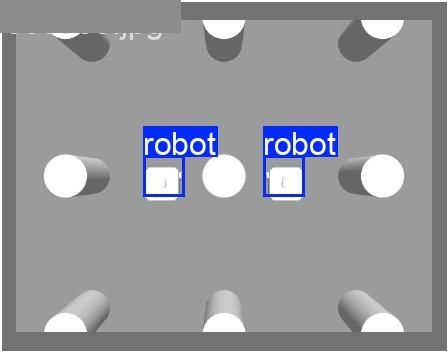
\includegraphics[width=0.85\linewidth]{fig_yolo_labels_crop.jpg}}
\centerline{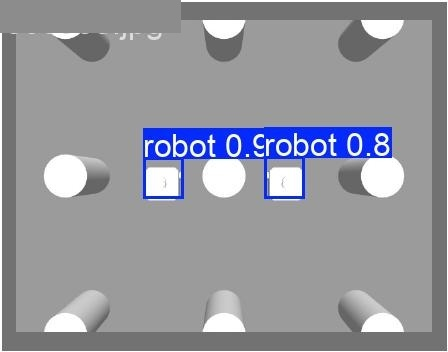
\includegraphics[width=0.85\linewidth]{fig_yolo_pred_crop.jpg}}
\caption{Dois dos robôs TurtleBot3 Waffle da frota vistos pela câmera cenital: anotação \textit{ground truth} (topo) vs.\ predição do detector (embaixo) em uma cena do conjunto de validação. Os experimentos completos com três robôs são quantificados nas Seções IV--V.}
\label{fig:robots}
\end{figure}

\begin{figure}[htbp]
\centerline{
\includegraphics[width=\linewidth]{fig_digitaltwin.png}}
\caption{Erro de localização do gêmeo digital ao longo de uma sequência contínua de rastreamento multi-robô. Erro médio de 4,7 cm; 100\% das detecções dentro de 15 cm do \textit{ground truth}.}
\label{fig:digitaltwin}
\end{figure}

Formulamos a alocação de tarefas como um Processo de Decisão de Markov (MDP): a cada chegada de demanda, um agente centralizado decide, com base no estado atual do sistema, qual dos $N=3$ robôs vai atendê-la. O estado de 21 dimensões descreve tudo o que o agente observa naquele instante: a posição $(x,y)$ de cada robô (do gêmeo digital ou da odometria, conforme o braço experimental), quanto tempo falta para cada robô ficar livre, a origem e o destino da demanda que acabou de chegar, e a origem e o destino das próximas duas demandas já visíveis na fila, um sinal de antecipação que permite ao agente considerar o impacto futuro de cada escolha, não só a demanda imediata. A ação é a escolha discreta de qual desses $N$ robôs deve atender a demanda atual. A recompensa é o tempo de resposta negativo $r = -(t_{\text{espera}} + t_{\text{deslocamento}})$: quanto mais rápido a demanda é atendida, da chegada até o robô escolhido começar a executá-la, maior a recompensa. Isso corrige uma formulação anterior que penalizava só o deslocamento até a demanda, ignorando quanto tempo o robô escolhido ainda levaria para ficar livre; sob essa formulação antiga, um robô ocupado e próximo podia parecer tão bom quanto um robô livre e distante, o que dava peso insuficiente aos efeitos de fila e enviesava a política para robôs livres, porém distantes. Treinamos com PPO~\cite{schulman2017proximal} via Stable-Baselines3~\cite{stable-baselines3} por 500.000 timesteps ($\sim$2h em CPU), nos hiperparâmetros padrão da biblioteca (Tabela~\ref{tab:hparams}) para isolar o efeito da fonte de observação e do masking, não o de ajuste fino do PPO; o Gazebo é reservado para validação física de estágio final, não para treino. Ambas as variantes de PPO aprendem (Fig.~\ref{fig:learning}): a recompensa média melhora de $\sim{-21}$ para $\sim{-17{,}7}$ ao longo de 500k passos, mas nenhuma cruza a linha de referência do nearest-free ($-16,7$); o PPO(odom) converge um pouco mais rápido, confirmando que o ruído de 4,7 cm do gêmeo digital é um efeito de segunda ordem.

\begin{table}[htbp]
\caption{Hiperparâmetros de treino (idênticos em todas as variantes)}
\begin{center}
\begin{tabular}{|l|c|}
\hline
\textbf{Hiperparâmetro} & \textbf{Valor} \\
\hline
Política / rede & MlpPolicy, $\pi$=[64,64], $V$=[64,64] \\
\hline
Taxa de aprendizado & $3\times10^{-4}$ \\
\hline
$n_{\text{steps}}$ (por ambiente) / batch & 2048 / 64 \\
\hline
$\gamma$ / GAE $\lambda$ / clip range & 0,99 / 0,95 / 0,2 \\
\hline
Ambientes paralelos / semente & 8 / 42 \\
\hline
\end{tabular}
\label{tab:hparams}
\end{center}
\end{table}

\begin{figure}[htbp]
\centerline{
\includegraphics[width=\linewidth]{fig_learning.png}}
\caption{Curvas de aprendizado do PPO para as variantes de observação YOLO e odometria, com o baseline nearest-free como linha de referência.}
\label{fig:learning}
\end{figure}

\section{Setup Experimental}

Comparamos o PPO contra três baselines: \emph{random} e \emph{round-robin}, que servem como piso de desempenho por não terem nenhuma noção de proximidade ou fila, e \emph{nearest-free}, que atribui o robô livre mais próximo e é inviável por construção quando nenhum robô está livre. Para isolar o efeito do gêmeo digital, treinamos PPO(YOLO) e PPO(odom), idênticos exceto pela fonte de posição usada na observação (ruído gaussiano de 4,7 cm no YOLO vs.\ drift acumulado de odometria no odom); usar sementes pareadas entre as duas variantes garante que a única diferença entre elas seja essa fonte de ruído, não a sorte do treino. Cada comparação avalia 1000 episódios pareados, usando a mesma sequência de demandas e semente para ambas as políticas, o que nos permite reportar não só se a diferença é estatisticamente significativa (Wilcoxon signed-rank) mas também seu tamanho de efeito (delta de Cliff) e incerteza (intervalos de confiança bootstrap). Para verificar se essas conclusões se sustentam sob diferentes pressões de demanda, um sweep de carga cobre seis regimes de intervalo entre chegadas, de 30s a 10s (500 episódios/ponto). O pipeline completo, da câmera ao YOLO, passando pelo alocador e pelo Nav2, até os robôs TurtleBot3 Waffle, foi validado de ponta a ponta em três robôs no Gazebo Classic (ROS2 Humble); a política de RL em si, porém, só é treinada no ambiente analítico. Para testar causalmente se a restrição suave de nunca atribuir um robô ocupado é a causa do desempenho ruim do PPO, treinamos também PPO(YOLO, masked): idêntico ao PPO(YOLO) exceto que a distribuição de ação é restrita, a cada passo, aos robôs atualmente livres, via \textit{action masking}~\cite{huang2022masking} usando o MaskablePPO da sb3-contrib, com os mesmos hiperparâmetros e orçamento de treino. Omitimos uma variante PPO(odom, masked) já que o efeito do ruído do gêmeo digital já se mostrou de segunda ordem (Seção~V), então testá-la não mudaria a conclusão qualitativa do experimento.

\section{Resultados}

A Tabela~\ref{tab:ablation} resume o desempenho em carga moderada. O nearest-free supera ambas as variantes de PPO nas três métricas de tempo (tempo de resposta médio, p95 e custo de resposta por episódio), em cerca de 12\% no tempo de resposta médio. Chama atenção que o PPO é \emph{melhor} na quarta métrica: ambas as variantes alcançam desbalanceamento de carga menor (0,135) que o nearest-free (0,149), indicando que a política de fato aprendeu a distribuir o trabalho de forma mais uniforme pela frota, mas que esse ganho não se converteu em atendimento mais rápido. A diferença entre PPO(YOLO) e PPO(odom) é pequena frente ao quanto qualquer uma das duas fica atrás do nearest-free, confirmando que o ruído do gêmeo digital é um efeito de segunda ordem. O teste de Wilcoxon confirma que essa vantagem é estatisticamente significativa em ambas as comparações ($p<0,001$, delta de Cliff grande). A razão p95/média é comparável entre as políticas ($\approx$1,47--1,56, Fig.~\ref{fig:boxplot}) e é, na verdade, ligeiramente menor para o PPO do que para o nearest-free. A desvantagem do PPO vem, portanto, de um deslocamento de toda a distribuição de tempo de resposta, e não de uma cauda de episódios catastróficos.

\begin{table}[htbp]
\caption{Comparação de políticas em carga moderada (inter-arrival 12s, 1000 episódios pareados). O tempo de resposta é espera + deslocamento; o custo de resposta é a soma dos tempos de resposta por episódio. Menor é melhor em todas as métricas.}
\begin{center}
\begin{tabular}{|l|c|c|c|c|}
\hline
\textbf{Política} & \textbf{Resp. média} & \textbf{Resp. p95} & \textbf{Custo resp.} & \textbf{Desbal.} \\
\hline
Nearest-free & \textbf{17,86 s} & \textbf{27,77 s} & \textbf{357,18 s} & 0,149 \\
\hline
PPO (YOLO) & 20,01 s & 29,46 s & 400,20 s & \textbf{0,135} \\
\hline
PPO (odom) & 19,83 s & 29,37 s & 396,69 s & \textbf{0,135} \\
\hline
\end{tabular}
\label{tab:ablation}
\end{center}
\end{table}

\begin{figure}[htbp]
\centerline{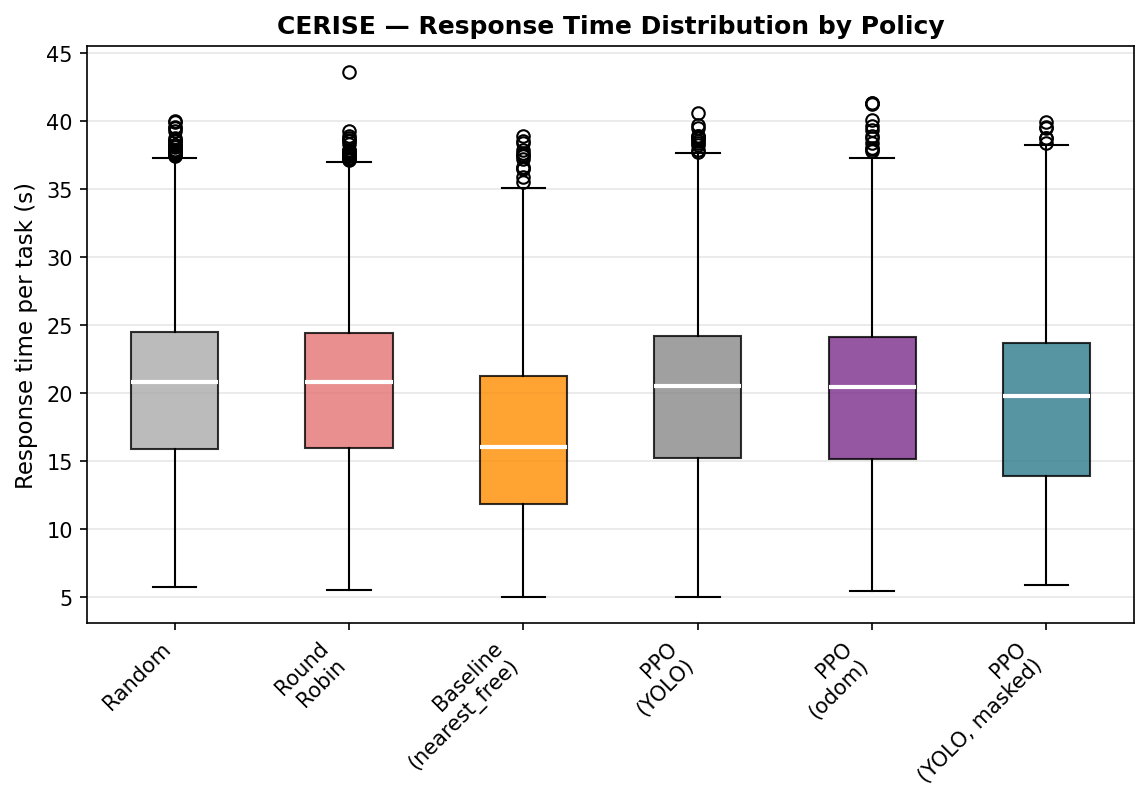
\includegraphics[width=\linewidth]{fig_boxplot.png}}
\caption{Distribuição de tempo de resposta entre as políticas avaliadas, incluindo a variante PPO mascarada.}
\label{fig:boxplot}
\end{figure}

A Tabela~\ref{tab:load} e a Fig.~\ref{fig:load} mostram que a desvantagem do PPO em relação ao nearest-free diminui conforme a carga aumenta, de +19,0\% em carga baixa para +7,7\% em carga alta, embora o nearest-free permaneça mais rápido em toda a faixa testada.

\begin{figure}[htbp]
\centerline{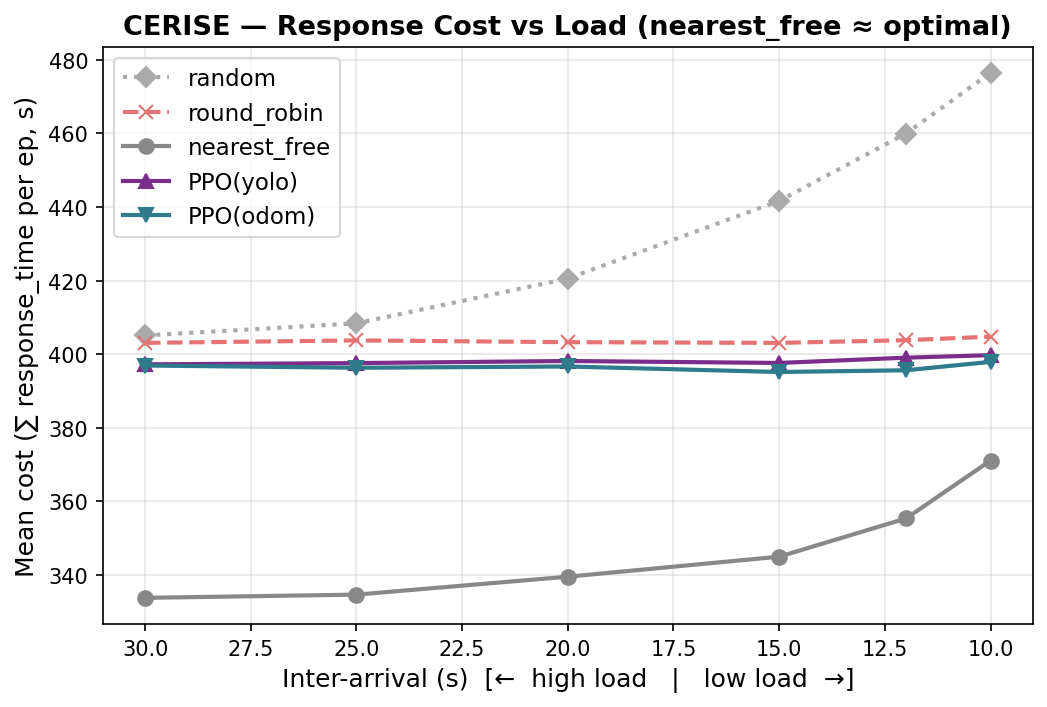
\includegraphics[width=\linewidth]{fig_load.png}}
\caption{Tempo de resposta em função da carga de demanda (inter-arrival) para nearest-free e PPO(YOLO).}
\label{fig:load}
\end{figure}

\begin{table}[htbp]
\caption{Tempo de resposta por política entre regimes de carga}
\begin{center}
\begin{tabular}{|l|c|c|c|}
\hline
\textbf{Inter-arrival} & \textbf{Nearest-free} & \textbf{PPO(YOLO)} & \textbf{Diferença} \\
\hline
30 s (baixa) & 333,8 s & 397,3 s & +19,0\% \\
\hline
12 s (mod.) & 357,2 s & 400,2 s & +12,0\% \\
\hline
10 s (alta) & 371,1 s & 399,8 s & +7,7\% \\
\hline
\end{tabular}
\label{tab:load}
\end{center}
\end{table}

\section{Diagnosticando o Resultado Negativo}

O PPO aprende, e ainda recebe um lookahead de duas demandas que o baseline guloso não tem, mas mesmo assim não supera o nearest-free. Investigamos três explicações. Imposição de restrição suave vs.\ rígida: o nearest-free nunca atribui um robô ocupado, pois essa restrição está embutida no próprio algoritmo; o PPO só consegue aprender a evitar isso indiretamente via penalidade na recompensa, e ainda assim erra em 4,2\% das decisões, contra 0,3\% do nearest-free, o maior contribuinte isolado que encontramos. Espaço de ação limitado: com apenas $N=3$ robôs, cada decisão oferece no máximo três alternativas, e poucas delas diferem de forma relevante no resultado, o que limita qualquer vantagem antecipatória que o lookahead poderia explorar. Orçamento de treino: 500k passos produziram aprendizado claro, mas não convergência, embora o próprio custo de resposta do PPO fique quase estável entre regimes de carga (397--400 s, Tabela~\ref{tab:load}) enquanto o do nearest-free cresce bastante em carga alta, sugerindo que o platô não é só um artefato de orçamento.

Teste causal. Para testar diretamente se essa violação de restrição era a causa, treinamos o PPO(YOLO, masked) e o reavaliamos junto com o PPO(YOLO) não-mascarado e o nearest-free sobre um novo conjunto de 1000 episódios em carga moderada, todos na mesma rodada de avaliação. O masking cumpre sua função por construção: a taxa de atribuição inválida cai de 4,0\% para exatamente 0,0\%. Mas o tempo médio de resposta melhora pouco, de cerca de 12\% pior que o nearest-free (não-mascarado) para cerca de 11\% pior (mascarado), uma melhora de aproximadamente 1 ponto percentual. O nearest-free ainda supera significativamente a variante mascarada ($p<0,001$, delta de Cliff $=0,636$), tamanho de efeito da mesma ordem de grandeza do não-mascarado ($\delta=0,703$).

A hipótese causal é refutada. A explicação que parecia mais plausível a priori não se sustenta: eliminar a violação por construção quase não fecha a diferença. O peso volta para o espaço de ação pequeno e o orçamento de treino, e surge uma explicação adicional: o masking remove não só a violação, mas também qualquer sinal de aprendizado sobre sua consequência, o que pode reduzir a diversidade de exploração da política sem compensar com vantagem real de antecipação. \textbf{Limitações.} Nossa alegação é delimitada por quatro escolhas. Primeiro, usamos hiperparâmetros padrão da biblioteca para o PPO, de modo que nosso resultado diz respeito ao PPO tal como comumente aplicado, e não ao teto do RL para este problema; um agente ajustado pode muito bem fechar a diferença. Segundo, $N=3$ robôs é um espaço de ação pequeno, e nosso próprio diagnóstico o aponta como fator dominante, de modo que estes achados não devem ser extrapolados para frotas grandes. Terceiro, a política treina em ambiente analítico e é validada de ponta a ponta no Gazebo, mas não em robôs físicos, de modo que a transferência sim-to-real permanece não testada. Quarto, 500k passos produziram aprendizado sem convergência. Cada um desses pontos é alvo direto dos trabalhos futuros.

\section{Conclusão e Trabalhos Futuros}

Integramos um gêmeo digital baseado em câmera, validado, a um alocador de tarefas multi-robô baseado em PPO, e constatamos que a política aprendida não supera uma heurística gulosa nearest-free. O action masking removeu o sintoma mais visível, uma taxa de atribuição inválida 13 vezes maior que a do baseline, sem recuperar a diferença de desempenho, o que aponta para o espaço de ação e o orçamento de treino.

A leitura prática é que, nesta escala, uma heurística gulosa já está próxima do que uma política aprendida consegue entregar, e sem custo de treino. Nossa varredura de carga sugere onde esse equilíbrio pode mudar: o custo de resposta do PPO permanece estável conforme a demanda cresce, enquanto o do nearest-free sobe, de modo que o ponto de cruzamento, se existir, está em carga mais alta ou frotas maiores do que testamos. Estabelecer se ele existe é o passo natural seguinte, e exige o espaço de ação maior e o orçamento de treino mais longo que nosso diagnóstico indica, além de uma arquitetura de política mais adequada à estrutura do problema que um MLP~\cite{agrawal2023rtaw,paul2022capsule}, validação física para além da simulação, e uma formulação como Dec-POMDP sob treino centralizado com execução descentralizada~\cite{lowe2017multi}.

\balance
\section*{Agradecimentos}
Os autores agradecem ao CERISE (Centro de Excelência em Redes Inteligentes Sem Fio e Serviços Avançados), sediado na Escola de Engenharia Elétrica, Mecânica e de Computação (EMC) da Universidade Federal de Goiás (UFG) e apoiado pela Fundação de Amparo à Pesquisa do Estado de Goiás (FAPEG), pela infraestrutura utilizada neste trabalho.

\begin{thebibliography}{00}
\bibitem{gerkey2004formal} B. P. Gerkey and M. J. Matarić, ``A formal analysis and taxonomy of task allocation in multi-robot systems,'' \textit{Int. J. Robot. Res.}, vol. 23, no. 9, pp. 939--954, 2004.
\bibitem{dias2006market} M. B. Dias, R. Zlot, N. Kalra, and A. Stentz, ``Market-based multirobot coordination: A survey and analysis,'' \textit{Proc. IEEE}, vol. 94, no. 7, pp. 1257--1270, 2006.
\bibitem{agrawal2022dcmrta} A. Agrawal, S. Hariharan, A. S. Bedi, and D. Manocha, ``DC-MRTA: Decentralized multi-robot task allocation and navigation in complex environments,'' in \textit{Proc. IEEE/RSJ Int. Conf. Intell. Robots Syst. (IROS)}, 2022, pp. 11711--11718.
\bibitem{pal2025together} A. Pal, A. Chauhan, and M. Baranwal, ``Together we rise: Optimizing real-time multi-robot task allocation using coordinated heterogeneous plays,'' in \textit{Proc. Int. Conf. Auton. Agents Multiagent Syst. (AAMAS)}, 2025.
\bibitem{lowe2017multi} R. Lowe, Y. Wu, A. Tamar, J. Harb, P. Abbeel, and I. Mordatch, ``Multi-agent actor-critic for mixed cooperative-competitive environments,'' in \textit{Proc. NeurIPS}, 2017.
\bibitem{henderson2018deep} P. Henderson, R. Islam, P. Bachman, J. Pineau, D. Precup, and D. Meger, ``Deep reinforcement learning that matters,'' in \textit{Proc. AAAI}, 2018.
\bibitem{orr2023survey} J. Orr and A. Dutta, ``Multi-agent deep reinforcement learning for multi-robot applications: A survey,'' \textit{Sensors}, vol. 23, no. 7, p. 3625, 2023.
\bibitem{yolov8} G. Jocher, A. Chaurasia, and J. Qiu, ``Ultralytics YOLO,'' 2023. [Online]. Available: https://github.com/ultralytics/ultralytics. Accessed: Jul. 15, 2026.
\bibitem{ahmed2021topview} I. Ahmed, S. Din, G. Jeon, F. Piccialli, and G. Fortino, ``Towards collaborative robotics in top view surveillance: A framework for multiple object tracking by detection using deep learning,'' \textit{IEEE/CAA J. Autom. Sinica}, vol. 8, no. 7, pp. 1253--1270, 2021.
\bibitem{huang2022masking} S. Huang and S. Ontañón, ``A closer look at invalid action masking in policy gradient algorithms,'' in \textit{Proc. Int. FLAIRS Conf.}, vol. 35, 2022.
\bibitem{schulman2017proximal} J. Schulman, F. Wolski, P. Dhariwal, A. Radford, and O. Klimov, ``Proximal policy optimization algorithms,'' 2017, arXiv:1707.06347.
\bibitem{stable-baselines3} A. Raffin, A. Hill, A. Gleave, A. Kanervisto, M. Ernestus, and N. Dormann, ``Stable-Baselines3: Reliable reinforcement learning implementations,'' \textit{J. Mach. Learn. Res.}, vol. 22, no. 268, pp. 1--8, 2021.
\bibitem{agrawal2023rtaw} A. Agrawal, A. S. Bedi, and D. Manocha, ``RTAW: An attention inspired reinforcement learning method for multi-robot task allocation in warehouse environments,'' in \textit{Proc. IEEE Int. Conf. Robot. Autom. (ICRA)}, 2023, pp. 1393--1399.
\bibitem{paul2022capsule} S. Paul, P. Ghassemi, and S. Chowdhury, ``Learning scalable policies over graphs for multi-robot task allocation using capsule attention networks,'' in \textit{Proc. IEEE Int. Conf. Robot. Autom. (ICRA)}, 2022, pp. 8815--8822.
\bibitem{dai2024dynamic} W. Dai, A. Bidwai, and G. Sartoretti, ``Dynamic coalition formation and routing for multirobot task allocation via reinforcement learning,'' in \textit{Proc. IEEE Int. Conf. Robot. Autom. (ICRA)}, 2024.
\bibitem{street2024right} C. Street, B. Lacerda, M. Mühlig, and N. Hawes, ``Right place, right time: Proactive multi-robot task allocation under spatiotemporal uncertainty,'' \textit{J. Artif. Intell. Res.}, vol. 79, pp. 137--171, 2024.
\bibitem{elfakharany2021endtoend} A. Elfakharany and Z. H. Ismail, ``End-to-end deep reinforcement learning for decentralized task allocation and navigation for a multi-robot system,'' \textit{Appl. Sci.}, vol. 11, no. 7, p. 2895, 2021.
\bibitem{fenoy2024attention} A. Fenoy, J. Zagoli, F. Bistaffa, and A. Farinelli, ``Attention for the allocation of tasks in multi-agent pickup and delivery,'' in \textit{Proc. ACM/SIGAPP Symp. Appl. Comput. (SAC)}, 2024, pp. 622--629.
\end{thebibliography}

\end{document}
